% Section 2 - Docker
% Roberto Masocco <roberto.masocco@uniroma2.it>
% May 1, 2022

% ### Docker ###
\section{Docker}
\graphicspath{{figs/section2/}}

% --- Docker Engine ---
\begin{frame}{Docker Engine}
\begin{columns}
  \column{.5\textwidth}
  \textbg{Docker} is the currently de-facto standard for building, managing and distributing \textbg{multiplatform} containers.\\
  It is an engine (i.e. a collection of \textbg{daemons}) that automates the management of the kernel subsystems in order to set up, store and run containers.

  \column{.5\textwidth}
  \begin{figure}
    \centering
    \label{fig:docker}
    
\includegraphics[scale=.2]{docker.png}
    \caption{Docker logo}
  \end{figure}
\end{columns}
\end{frame}
\begin{frame}{Docker Engine}
\begin{figure}
  \centering
  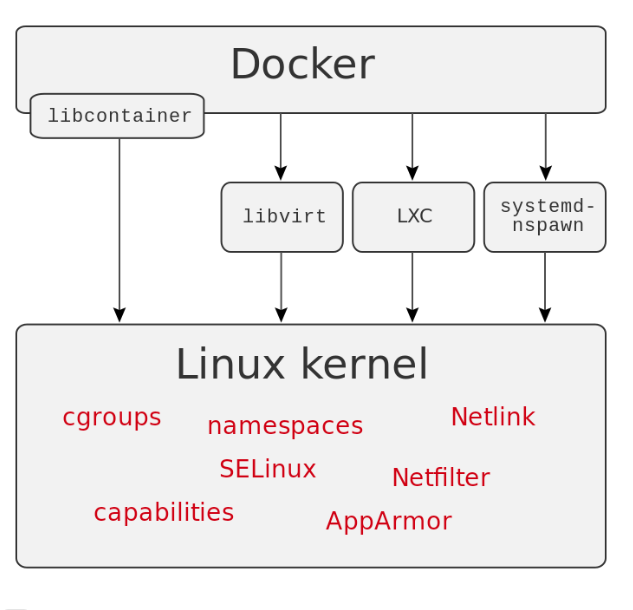
\includegraphics[scale=.3]{dockerScheme.png}
  \label{fig:dockerscheme}
  \caption{Docker Engine scheme}
\end{figure}
\end{frame}

% --- Containers in Robotics ---
\begin{frame}{Containers in Robotics}
Containers can be of help in some classic scenarios:
\begin{itemize}
  \item \textbg{deploying} applications or whole control architectures, solving issues like \textbg{dependencies} and \textbg{configurations};
  \item configuring and distributing \textbg{development environments};
  \item expanding the capabilities of \textbg{(partially) closed-source} hardware solutions (e.g. Nvidia Jetson...).
\end{itemize}
\end{frame}
